%!TEX root = main.tex
\chapter{Our Approach}

This section introduces our approach for modeling a \acf{DFP} as a \acf{CSP} and reaching a valid solution. We describe how we modelled the problem as a \ac{CSP}, the methodologies used to analyze and extract the information from the digital evidences, the structures used to model the problem and how they are used to reach a solution.

\section{Introduction}

After seeing what a \ac{DFP} and a \ac{CSP} are we can finally start modelling a \ac{DFP} as a \ac{CSP} to try to reach a valid solution. Like mentioned in previous chapters there are a lot of constraint programming tools, but the one we ended up using was Choco Solver~\cite{chocoSolver}. Along with Choco Solver, we also used the \ac{TSK}~\cite{tsk} framework mentioned previously.

\section{Methodology}

After acquiring the disk image to be analyzed, it is first processed with the help of tools from the \ac{TSK} framework, first with Sorter, that can take an hash database form the NIST National Software Reference Library, or NSRL for short, that contains all the signatures of traceable software applications (this way we can shorten at the start the number of \INODES that are known to be safe). The sorter creates multiple files with different names, each name being a pre-determined type of file, such as archive, executable or data. After the sorter finishes running, we run Mactime, and it creates a single file containing time information about every file present in the file system. Examples of these files can be seen in Figure~\ref{fig:sorterOut} and Figure~\ref{fig:mactimeOut}. 

\begin{figure}[ht]
    \centering
    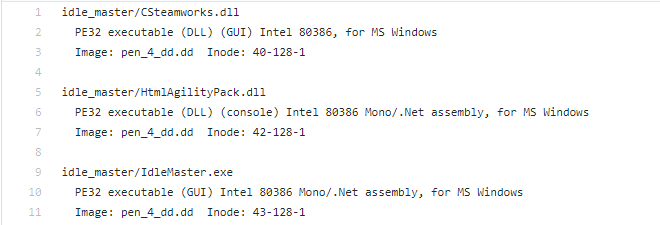
\includegraphics[width=120mm]{sorter_out.png}
    \caption{Example of Sorter output for executable files}
    \label{fig:sorterOut}
\end{figure}

\begin{figure}[ht]
    \centering
    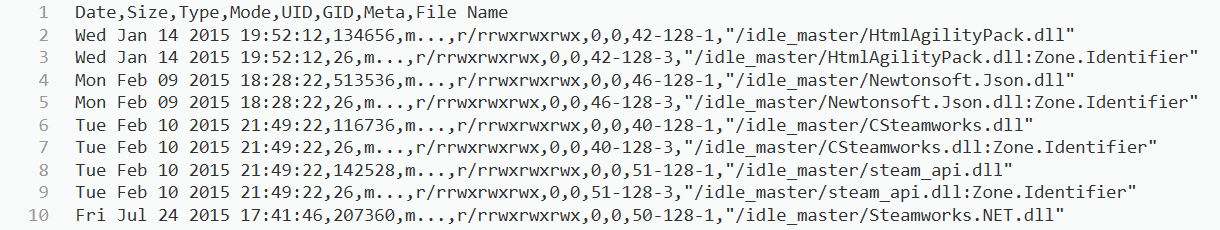
\includegraphics[width=120mm]{mactimeOut.png}
    \caption{Example of Mactime output for a 4GB pen drive}
    \label{fig:mactimeOut}
\end{figure}

The files created by Sorter include all relevant information about the files present in the file system that is being analyzed, including: file path in the file system, the file type, the image name (from where the data was extracted) and the \INODE number, which is an internal representation of that particular file in the file system. As for the Mactime file, it only contains date information about each file. This information is parsed into a database that allows the data to be persistent. This database is described in detail in Section~\ref{dbcache}. The data also passes through a caching system that tries to determine if the exact type of constraints have been applied to the file system being analyzed to find if it can skip the lengthily process of trying to find a solution. The caching system is described in detail in Section~\ref{dbcache}.

The whole program can be shortened into the small flow diagram seen in figure \ref{fig:diagram}.

\begin{figure}[h]
    \centering
    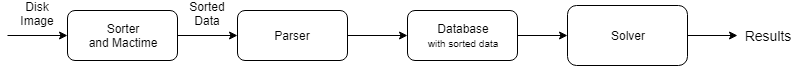
\includegraphics[width=120mm]{diagram.png}
    \caption{Flow diagram}
    \label{fig:diagram}
\end{figure}

After pre-processing the disk image and persisting all necessary data, the \ac{DFP}, which describes the items that being looked for, is modeled as a \ac{CSP}. This \ac{CSP} is then solved by a \ac{CSP} solver, to reach a solution that satisfies the initial \ac{DFP}, if it exists. A solution to such a \ac{CSP} will be a set of file identifiers that match the \ac{DFP}. It is necessary to use specific constraints to reach the solution mentioned before, which are used to restrict the domain of the variables. These constraints are described in Section~\ref{Constraints}.

\section{Modeling}

The problem is modeled as a set of variables that represent the files that need to be found, according to the \ac{DFP}. These files are represented as numerical values, which are the \INODE numbers extracted from the Sorter mentioned previously. Each of these variables are associated with a domain and a set of constraints which are applied to the variables. As previously stated these constraints were created specifically in the context of this work.

In this work we use the Choco Solver, which allows the use of four different types of variables to model the problems: Integers (IntVar), Booleans (BoolVar), Sets (SetVar) and Reals (RealVar). To model a \ac{DFP} as a \ac{CSP}, we decided to use Set variables (SetVars). Although the problems are always modelled with one variable, that doesn't mean we will only have one solution, in fact, SetVars can be instantiated to several values at the same time.

In Choco Solver, SetVars are defined by a domain that is made of two other domains, the Lower Bound (LB) and the Upper Bound (UB). The Lower Bound is a set of integers that must belong to every solution, while the Upper Bound is composed of the set of integers that may be part of the final solution~\cite{SetVar}. In our case, when creating the variable with which we are going to work with, the Lower Bound will be left empty. As for the  Upper Bound, it will be composed of all the \INODES found during the parsing phase.

\floatname{algorithm}{Listing}

\begin{algorithm}
    \caption{Modelling of a Digital Forensics \ac{CSP}}
    \label{modelling}
    \begin{algorithmic}
        \State{}
        \State{$CSP = (V, D, C)$}
        \State{}
        \State{$V =\{V_1,V_2,\ldots,V_n\}$}
        \State{}
        \State{$D = \{D_1,D_2,\ldots,D_n\},\quad \forall D_i \in D : D_i = \{Y_1,Y_2,\ldots,Y_z\}$}
        \State{}
        \State{$C=\{C_1(V_i,\ldots,V_j),\ldots,C_k(V_i,\ldots,V_j)\},$}
        \State{$\qquad \qquad \qquad \qquad \qquad \forall C_k \in C : C_k = \{CP_1(V_i,\ldots,V_j),\ldots,CP_z(V_i,\ldots,V_j)\}$}
        \State{}
    \end{algorithmic}
\end{algorithm}

Listing~\ref{modelling} presents a formal representation of a digital forensics \ac{CSP}, represented by the triple $CSP = (V,D,C)$. $V$ is the set of variables, which represents the files to be found, $D$ is the set of domains for each variable which, where each $D_i = \{Y_1,Y_2,\ldots,Y_z\}$ is a set of integer values that represent the \INODES present in the file system; and $C$ is the set of constraints which restricts the domain of each variable, where each $C_k$ is mapped into a specific constraint propagator.

\section{Constraints}
\label{Constraints}

To reach a solution, Choco solver makes use of constraints which are implemented as propagators. A propagator declares a filtering algorithm that can be applied to the variables that models the problem, in order to reduce their domain~\cite{Propagator}. In the context of this work, we implemented the following propagators:

\begin{enumerate}
    \item \textbf{File type:} restricts the domain according to the given type of file.
    \item \textbf{File path:} restricts the domain according to the given path.
    \item \textbf{Word search:} restricts the domain according to the given word.
    %\item \textbf{NIST:} restricts the domain according to the NIST database.
    \item \textbf{Date:} restricts the domain according to the given date.
\end{enumerate}

All these propagators were implemented to work with the variables used to model the problem: SetVar.

To create the propagators, we had to implement the following methods: \texttt{propagate} and \texttt{isEntailed}. The method \texttt{propagate} should restrict the domain according to what we need, while the method \texttt{isEntailed} informs the propagator if a problem has a solution or not, or if it is not possible to determine if a solution exists. These methods are described in detail in Listings~\ref{propagate} and~\ref{isEntailed}.

\floatname{algorithm}{Listing}

\begin{algorithm}
    \caption{propagate method}
    \label{propagate}
    \begin{algorithmic}
        \For{each value in UB}
            \If{value not in database}
                \State{Remove value from UB}
            \EndIf
        \EndFor
    \end{algorithmic}
\end{algorithm}

\begin{algorithm}
    \caption{isEntailed method}
    \label{isEntailed}
    \begin{algorithmic}
        \If{UB is empty}
            \State{Problem is impossible to solve}
        \Else
            \State{Problem has possible solution}
        \EndIf
    \end{algorithmic}
\end{algorithm}

\subsection{Type, Path and Date Propagators}

The Type propagator was the first propagator created and it takes the Upper Bound of the SetVar, iterates over it and removes any \INODE that does not belong to the type we are looking for. Path and Date propagators work in the same way. The main difference is what they are trying to restrict: the Type propagator receives the type of file we want to restrict and iterates over the Upper Bound to remove every \INODE that does not belong to that type of file, while the Path propagator receives a path and, similarly to the Type propagator, iterates over the Upper Bound and removes every \INODE that does not belong to that path. An implementation in pseudo-code of these propagators can be seen in Listing~\ref{propagators}.

The type and path propagators have a separate definition that can take more than one input at a time. The separate definition of the type propagator can take more than one type of file so we can look for more than type at a time and the separate definition for the path propagator can take more than one path to search on different folders at the same time.

\floatname{algorithm}{Listing}
\begin{algorithm}
    \caption{Type, path and date propagator}
    \label{propagators}
    \begin{algorithmic}
        \For{var $\in$ UB}
            \State{Q $<=$ \{Query the database if var is of given type, path or date\}}
            \If{Q is null}
                \State{Remove var from UB}
            \EndIf
        \EndFor
    \end{algorithmic}
\end{algorithm}

\subsection{Word Search Propagator}

This propagator relies on the Unix4j~\cite{Unix4j} Java library. This library implements most of the Unix shell commands in native Java. We use this library since it provides efficient methods to find contents inside a file in any file system. The main method we use from this library is the implementation of the Unix Grep command. We decided to use Grep because we needed a fast and efficient method to search for words in files and seeing as the bash already had a very powerful tool to achieve what we wanted we found the Unix4j Library which permitted us to use bash commands without being in a native Unix environment.

This propagator works in a similar way to the ones previously described. It iterates over the Upper Bound and removes any file that does not contain the word we passed as argument. Also, since this is the last constraint ever being run, we add the \INODES that passed through the propagator to the Lower Bound, because at this moment we're certain these will belong to the final solution. An implementation of this propagator can be seen in pseudo-code in Listing~\ref{wordSearch}.

\floatname{algorithm}{Listing}
\begin{algorithm}
    \caption{Word Search Propagator}
    \label{wordSearch}
    \begin{algorithmic}
        \For{var $\in$ UB}
            \State{\INODE $<=$ \{Query database to retrieve var information\}}
            \If{I not null}
                \If{[\INODE -> name] contains "word"}
                    \State{Add var to LB}
                \Else
                    \State{G $<=$ \{grep -c [\INODE => path]\}}
                    \If{G $=$ 0}
                        \State{Remove var from UB}
                    \Else
                        \State{Add var to LB}
                    \EndIf
                \EndIf
            \EndIf        
        \EndFor
    \end{algorithmic}
\end{algorithm}

\section{Data Persistence \& Caching}
\label{dbcache}

In an initial developing phase, the database system didn't exist, and data wasn't persisted at all.
The \INODES where stored in data structures like Hashtables and Linked Lists, and later transferred directly into the array used as the domain of the SetVar used as our variable. This was extremely inefficient, every time we wanted to test a part of the code we would have to run the whole thing and parse the whole information from the Sorter output files, this ended up being one of the reasons why we changed the initial structure of the program.

As mentioned before, we decided to use a database to persist data in the case of re-running the code over the same device. This database is created at the time of parsing the data. If the data has not been parsed before, a new database is created for the data being parsed, it can have multiple stored databases for different devices. The database contains five things: 1) the file id (the \INODE number); 2) the file name; 3) the file path; 4) the file type and 5) the file date (from the Mactime output).

The caching system was created to lessen the time it takes for the system to solve all the constraint problems it was commissioned to solve by searching in a data structure that contains all the results of previous constraint problems, including the ones that have no results. Every time the system is initiated, it checks if what we're trying to solve has been solved before, and if so, it skips the whole constraint process and just gives us the results we want, if not it runs like normal and saves the results at the end. This applies to all combination of constraints. These results are being saved in a simple key-value data structure, a hashtable.



